\section{Uvod}
\label{sec:uvod}

Mnogi kompajleri obavljaju neki deo svog rada pomoću očuvanja ispravnosti, poboljšanja performansi, programskih transformacija. Radi konkretnosti, fokusirali smo se na Glazgov Haskel Kompajler (eng. \emph{Glazgov Haskell Compiler (GHC)}), ali ističemo da sve što navedemo u ovom radu je primenljivo i za bilo koji kompajler za funkcionalni jezik, a možda i
na kompilaciju za druge jezike. GHC preuzima ovu ideju “kompilacije transformacijom” pokušavajući da što više izrazi proces kompilacije u obliku programskih transformacija. U ovom radu prikazaćemo u primeni transformacione tehnike kroz GHC kompajler za funkcionalni jezik Haskel (eng. \emph{Haskell}).

\subsection{Haskel}
\label{subsec:podnaslovHaskel}
Haskel je funkcionalni jezik opšte namene, koji sadrži mnoge inovacije u dizajnu programskih jezika. Haskel podržava funkcije višeg reda (eng.\emph{ higher-order functions}), ne-striktnu semantiku, statički polimorfizam, korisnički definisane algebarske tipove, prepoznavanje šablona (eng. \emph{ pattern-matching}), rad sa listama. Razvijen je kroz sistem modula kao proširenje programskog jezika. Poseduje veliki skup primitivnih tipova uključujući liste, nizove, cele brojeve različitih namena i dužina, realne brojeve. Može se reći da je Haskel zavšetak dugogodišnjeg rada i istraživanja na ne-striktnim funkcionalnim jezicima. 

\subsection{GHC}
\label{subsec:podnaslovGHC}

Uobičajno se tretira kao standardna implementacija Haskela, na kojoj se baziraju i druge implementacije. Razvijan je počev od 1989. godine. GHC je pisan u Haskelu – kompajler sadrži 227,000 linija k\hat{o}da (uključujući komentare), a biblioteke (moduli) sadrže 242,000 linija k\hat{o}da (uključujući komentare).

Sastavni deo svakog kompajlera za funkcionalni jezik čini i run-time sistem. Za GHC, run-time sistem je pisan u C-u i sadrži 87,000 linija k\hat{o}da.

Tekuću verziju kompajlera, razvijalo je 23 istraživača (eng. \emph{developers}) sa preko 500 priloga (eng. \emph {commits}).

Celokupna struktura kompajlera se sastoji iz tri faze :
\begin{enumerate}
	\item Prva faza (eng. \emph{Frontend}) čini pretvaranje izvornog k\hat{o}da pisanog u Haskelu, u takozvani Core jezik (eng. \emph {Core language}). U ovoj fazi, kompajler napisan u Haskelu, vrši analizu izvornog k\hat{o}da, pravi odgovarajuće drvo izvođenja, realizuje leksičku i sintaksnu analizu, proveru tipova i kao izlaz daje k\hat{o}d sa veoma redukovanim skupom instrukcija, koji zahteva Core. Više o ovoj fazi može se naći u Sekciji \ref{sec:frontend}.
	\item Druga faza (eng. \emph {Middle End}) – izlazni k\hat{o}d iz prethodne faze – međujezik (eng. \emph {Intermediate language)}) se dodatno optimizuje, i to kroz niz transformacija. Rezultat rada Core-a se dobija u Core obliku. Na taj način, sledeće etape transformacije k\hat{o}da tačno znaju kakve konstrukcije im se mogu naći na ulazu.  Više o ovoj fazi može se naći u Sekciji \ref{sec:middle}.
	\item Treća faza (eng. \emph {Backend}) obuhvata generisanje k\hat{o}da. Core-ov k\hat{o}d iz prethodne faze postaje ulaz u STG-mašinu (eng. \emph {Spineless Tagless G-machine}). Rezultat rada STG-mašine se grana u tri toka. Prvi tok podrazumeva prevođenje u izvorni mašinski k\hat{o}d. Drugi tok podrazumeva korišćenje LLVM-a za dobijanje optimizovanog k\hat{o}da pomoću ove virtualne mašine. Treći tok koristi jezik C-\,- za dobijanje izvršnog k\hat{o}da. Više o ovoj fazi može se naći u Sekciji \ref{sec:backend}.
\end{enumerate}

Razvojne etape pravljenja izvršnog k\hat{o}da mogu se videti na slici \ref{fig:razvojneEtaple}.

\begin{figure}[h!]
	\begin{center}
		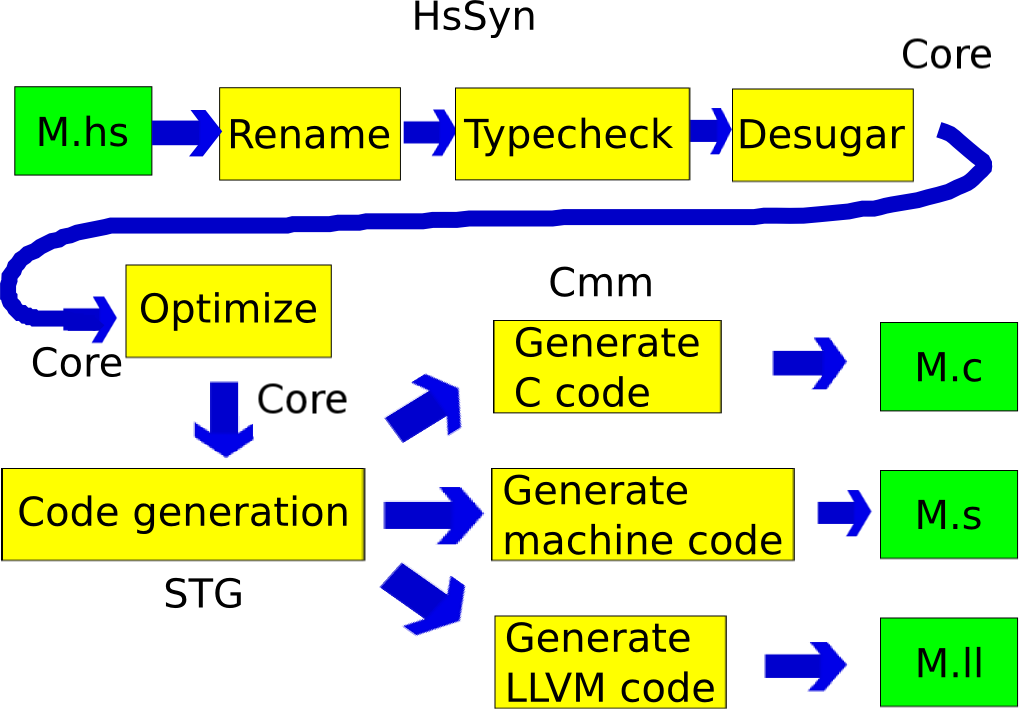
\includegraphics[scale=0.30]{resources/razvojneEtape.png}
	\end{center}
	\caption{Razvojne etape pravljenja izvršnog k\hat{o}da}
	\label{fig:razvojneEtaple}
\end{figure}